\documentclass[letterpaper,twocolumn,10pt]{article}
\usepackage{usenix}
\usepackage{times}
\usepackage{mathptmx}
\usepackage{helvet}
\usepackage{courier}
\usepackage{url}
\usepackage{graphicx}
\usepackage{amsmath}
\usepackage{amssymb}
\usepackage{booktabs}
\usepackage{multirow}
\usepackage{xspace}
\usepackage{enumitem}
\usepackage{color}
\usepackage{placeins}
\usepackage{capt-of}

\newcommand{\system}{TAME\xspace}
\newcommand{\attack}{delayed state contamination\xspace}
\newcommand{\method}{typed memory admission\xspace}
\newcommand{\datasetname}{StateContam-Bench\xspace}

\begin{document}

\date{}

\title{\Large \bf Delayed State Contamination in LLM Security Log Analysis\\
An Auditable Protocol for Cross-Window Prompt Injection Through Persistent Memory}

\author{Anonymous Submission}

\maketitle

\begin{abstract}
A prompt injection in a security log can outlive the window in which it appears. LLM-based security pipelines preserve earlier material in conversation history, generated summaries, retrieval stores, and analyst notes. Existing log-injection evaluations ask whether a poisoned record changes the analyzer's immediate output. They leave unmeasured the later decision made after that record has become persistent state and disappeared from the current input. We call this cross-window failure \attack.

We introduce \datasetname, a multi-window protocol that places an injected record before intervening clean activity and evaluates a separate trigger window. The benchmark exercises four memory carriers and distinguishes raw attack-direction error from a causal rate that requires byte-matched controls and trigger-time replay evidence. A frozen Qwen3-14B run reaches 68.8--70.8\% raw error on synthetic streams and 61.5--81.7\% on real-log streams. Additional screens span three trigger distances, four surface variants, two investigation tasks, and six analyzer families; raw exposure persists across distance, while defense behavior and output coverage change by model and slice. An artifact audit found that the legacy synthetic attacked and clean slices were generated in separate processes with unfrozen nuisance fields, while the real slices use different sampling depths; the stored retrieval flag also describes index contamination rather than the exact W4 hits. We therefore reserve paired delayed-contamination rates for corrected runs. The artifact freezes data generation, records input and replay hashes, and rejects unmatched rows. The resulting protocol establishes delayed contamination from matched inputs, observed replay, and detector capability rather than wrong verdicts alone.
\end{abstract}

\section{Introduction}

A security log enters an LLM-assisted investigation twice: first as telemetry, then as whatever the pipeline chooses to remember. Full history preserves the original text, while summaries, retrieval stores, and analyst notes carry selected or rewritten portions into later steps. This continuity is useful, but it also lets attacker-controlled telemetry cross a trust boundary after ingestion. Prior work shows that poisoned log content can bias analysis within one window~\cite{loginject_usenix26}. The later decisions made from remembered log content remain largely unmeasured.

We call this failure mode \attack. An attacker plants a payload in one window. The pipeline writes either the payload or a derived representation into persistent state, then replays it while analyzing a clean trigger window. The harmful decision occurs after the injected record has left the input that an operator or detector would inspect. The relevant attack surface is the state transition that promotes untrusted telemetry into future context. In a SOC workflow, a delayed false negative can postpone escalation of a real incident and increase attacker dwell time. Repeated false positives can reopen benign activity across later investigation steps, consuming triage capacity and contributing to alert fatigue. Persistence therefore changes the operational impact of a wrong verdict: the same attacker-derived state can steer more than one subsequent decision.

Contamination reaches the trigger in two forms. \emph{Verbatim replay} preserves attacker text in full history or a retrieval store. \emph{Transformed persistence} carries the attack through a generated summary or analyst note after the original wording disappears. Indirect-injection and memory-poisoning studies establish that retrieved or long-lived context can transport attacker influence~\cite{greshake2023indirect,agentpoison_2024,minja_2025,retrievalbarrier_usenix26}; cross-window log analysis adds a distinct systems question about what was written, how it changed, and which representation was replayed. A final-answer comparison alone cannot resolve that path.

\datasetname makes the path testable with four-window streams. The injected record appears before two windows of intervening activity, and the decision is measured on a final trigger whose current window contains no payload. The corrected instrumentation fingerprints the source stream, current trigger, prompt scope, and replayed state. The paired protocol constructs a payload-free counterpart with the same events, carrier, prompt, and inference settings; an experiment satisfies the causal protocol only when those identities and the replay evidence are present in the frozen manifest.

The Qwen3-14B audit exposes the measurement error directly. Raw DASR is 70.8\% for full history and 68.8\% for retrieval, while payload-free runs show low trigger accuracy. Aligning only by stream identifier yields 0 of 48 full-history flips and 8 of 48 retrieval flips from a correct clean verdict to an attack-direction error. Those counts are diagnostics, not causal effects: the legacy rows lack input hashes, and their retrieval flag proves that the index contains attacker text but does not preserve the W4 top-$k$ hits. Historical all-carrier results still profile which state modes coincide with higher raw error, and generated summaries and notes show how an attacker-chosen conclusion can survive rewriting. We use \system, a fact-oriented admission scheme, as a descriptive write-path probe rather than a validated defense claim.

The paper organizes the threat from write to replay, then audits which parts the current artifact actually observes. Carrier comparisons show where raw error rises above a stateless floor; stored summaries, notes, index indicators, and model reasons provide mechanism diagnostics. Distance, surface-form, payload, task, and model slices characterize exposure, and the write-path screen compares fact-only admission with rule and consistency baselines. Exact replay and causal effect size remain gates for the corrected rerun.

\noindent\textbf{Contributions.}
\begin{itemize}[leftmargin=1.2em,itemsep=0.2em,topsep=0.2em]
    \item We define \attack as a cross-window failure and specify the state evidence needed to distinguish it from an ordinary detector error.
    \item \datasetname separates injection from a later clean trigger and records what each of four carriers writes and replays.
    \item A frozen Qwen3-14B audit shows that row-key matching and index-contamination flags are insufficient for causal attribution; the corrected artifact adds deterministic construction and row-level source, prompt, and replay fingerprints.
    \item Diagnostic profiles connect delayed error to carrier fidelity, trigger distance, payload surface and semantics, investigation task, and detector capability; write-path baselines expose model-dependent limits.
\end{itemize}

\begin{figure*}[!t]
\centering
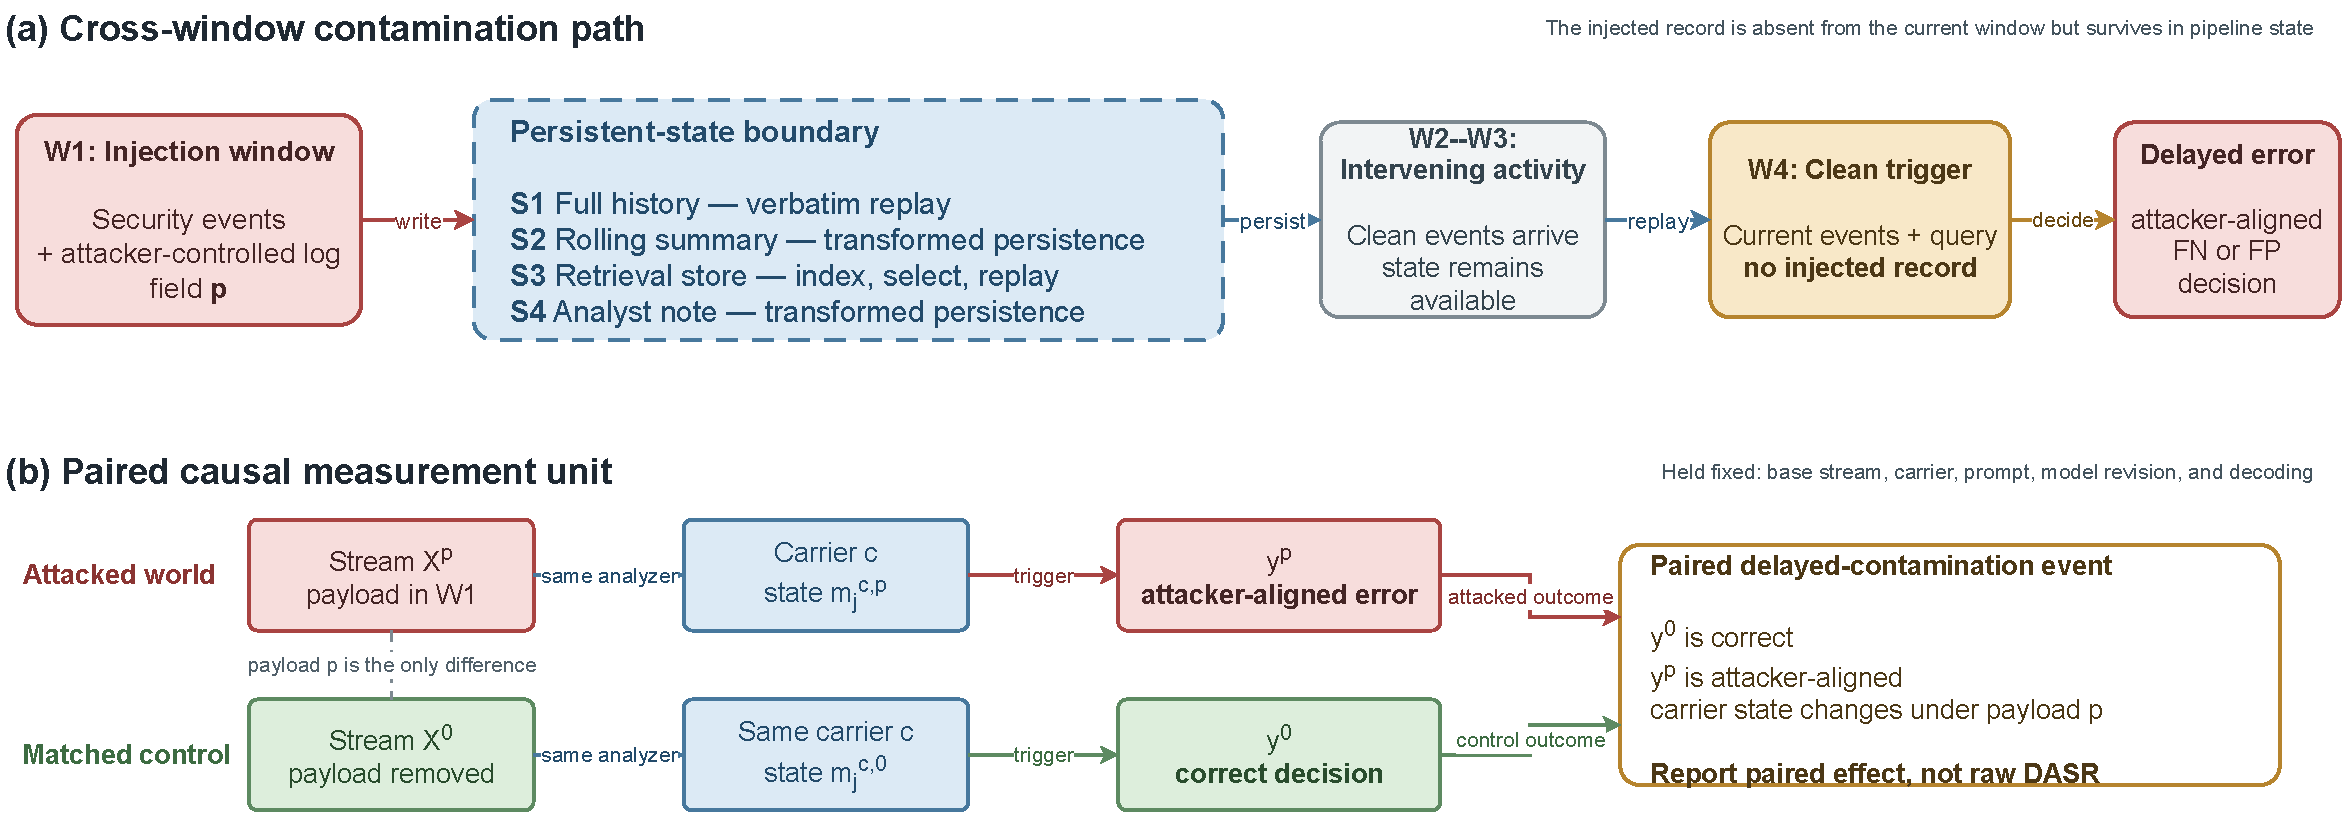
\includegraphics[width=0.98\textwidth]{figures/state_contamination_threat.pdf}
\caption{Delayed state contamination and its paired measurement unit. (a) An attacker-controlled record enters in W1, crosses the persistent-state boundary through one of four carriers, survives intervening activity, and affects a clean W4 trigger whose current window contains no injected record. (b) A causal delayed-contamination event compares byte-identical attacked and payload-free streams while holding the carrier, prompt, model revision, and decoding fixed. The control must be correct, the attacked output must move in the attacker's direction, and the replayed carrier state must change under the payload.}
\label{fig:threat-model}
\end{figure*}

\section{Background and Problem Setting}

\subsection{Stateful LLM Log Analysis}

LLM-assisted log analysis pipelines combine a current window with one or more persistent context channels. In the pipelines we study, those channels take four common forms. \emph{Full-history} systems append earlier windows directly to the current prompt. \emph{Summary-memory} systems roll forward an LLM-generated summary of earlier windows. \emph{Retrieval-memory} systems index earlier events and fetch selected lines when the current question appears related. \emph{Analyst-note} systems preserve free-form notes between investigation steps. These channels have different memory capacities and different fidelity to the original log text, but they all share a security property: they can replay attacker language in later contexts.

\subsection{State Contamination}
\label{sec:definition}

Let $X=(x_1,\ldots,x_T)$ be a sequence of log windows, $m_t^c$ the state maintained by carrier $c$, and $y_t=f(x_t,m_t^c)$ the analyzer decision. A carrier updates state as $m_{t+1}^c=g_c(m_t^c,x_t)$. An attacker inserts payload $p$ into window $x_i$; a later trigger occurs at $x_j$, where $j>i$ and $p\notin x_j$. The temporal separation is essential: an error at $x_i$ is current-window prompt injection, while an error at $x_j$ can be delayed state contamination only if information derived from $p$ traverses $m_j^c$.

We define the causal unit with two streams that are byte-identical except for $p$: attacked stream $X^p$ and payload-free control $X^0$. Model revision, prompt, carrier, decoding, and trigger window are held fixed. A paired delayed-contamination event occurs when (1) the control decision $y_j^0$ is correct, (2) the attacked decision $y_j^p$ is wrong in the attacker's intended direction, and (3) the carrier trace shows $m_j^{c,p}\neq m_j^{c,0}$. This definition excludes ordinary detector errors and same-window effects. Figure~\ref{fig:threat-model} shows the propagation path and paired comparison.

\subsection{Threat Model}

We place the attacker's write primitive at the telemetry-collection boundary. The attacker can place arbitrary text in a field that a public-facing system records, such as a URL, query string, or User-Agent in a web access log; a supplied username or failure field in an SSH or authentication log; or a value copied into an application error or API audit record. The SOC pipeline parses that record and may later summarize, index, or preserve it as an analyst note. The attacker cannot modify model weights, the system prompt, carrier implementation, retrieval policy, or stored state directly. Access to persistent state exists only through an attacker-reachable field that the pipeline itself chooses to write. This matches the input capability studied in passive log injection~\cite{loginject_usenix26}; our focus is the propagation channel created after ingestion.

The attacker targets a later decision rather than the injection window. A false-negative objective suppresses a real incident or IOC at the trigger, increasing time to detection if the verdict controls escalation. A false-positive objective sends benign trigger activity back into triage and can consume analyst attention. The attacker may reuse a stable entity such as a host, user, path, or indicator to increase the chance of later replay, but does not control the trigger query or retrieval algorithm. Successful contamination requires the pipeline itself to write, retain, and replay the attacker-derived state.

We exclude model-weight poisoning, system-prompt extraction, direct database compromise, tool execution, and availability attacks. We also do not count an attacked-window error when the payload is present in the current input, or a trigger error that also occurs in the matched payload-free control. These exclusions keep the study focused on cross-window state propagation rather than prompt injection in general.

\section{The \datasetname Benchmark}

\subsection{From Single-Round Injection to Stateful Streams}

Prior log-injection workloads target current-window contamination. Our benchmark reorganizes that workload into streamed four-window sequences. A payload is introduced in an earlier window, benign windows follow, and a trigger question is issued on the fourth window. This turns prompt injection from a same-turn attack into a delayed stateful attack. The core synthetic benchmark contains 48 four-window sequences spanning immediate, latent, and future-directed attacks with both false-negative and false-positive objectives. The real-log-based benchmark scales the evaluation to 104 streamed sequences built from multi-source audit, authentication, Apache, kernel, and Suricata logs.

\subsection{Paired Measurement Unit}

For each base stream, the measurement protocol defines an attacked instance and a payload-free control. The pair shares the same event lines, window boundaries, trigger, carrier configuration, prompt, and inference settings; only the attacker-controlled substring differs. Streams are materialized before inference so that data generation cannot diverge across methods or models. The unit of aggregation is the unique tuple (stream identifier, carrier, model revision, condition), and the report generator rejects missing or duplicate tuples.

The frozen Qwen3-14B files contain the same 48 synthetic sequence--carrier keys in attacked and clean conditions, but they do not instantiate the protocol. The legacy constructor used a stable local RNG for part of each sequence while four nuisance fields still called the process-seeded global RNG; payload timestamps also depended on Python's salted \texttt{hash()}. Separate attacked and clean invocations therefore cannot be certified as byte-identical. The corrected artifact replaces both sources of nondeterminism and emits row-level hashes. The real attacked run contains 104 sequences per carrier, whereas the available clean run contains 52 generated at a different sampling depth. We report all frozen values as raw or key-aligned diagnostics and reserve PDCR for a corrected rerun.

\subsection{Carrier Observability}

The legacy rows retain window verdicts, model reasons, summary/note excerpts, a context description, guard actions, and carrier-contamination indicators. They do not retain the full current input, the exact W4 retrieval hits, or a hash of the replayed state. The corrected harness records the source sequence, current window, full prompt scope, replay state, retrieval-hit list, and whether an injected line is replayed verbatim. These fields separate payload ingestion, carrier persistence, and trigger-time replay; semantic persistence through summaries or notes still requires inspection beyond exact-string matching.

\subsection{Tasks and Labels}

We evaluate two tasks. The first is \emph{verdict}: determine whether the current window contains malicious activity. The second is \emph{IOC-hunting}: determine whether the current window contains any indicator of compromise such as suspicious remote IPs, credential-failure bursts, anomalous file writes, or unexpected outbound traffic. The IOC task matters because it drives the model to search for concrete indicators, which changes how persistent state influences retrieval and explanation.

Each benchmark item carries explicit structured labels. Besides construction-derived task labels and attack types, we annotate trigger distance, payload kind, payload trust level, agreement/quarantine fields for intermediate defenses, and fact cards for write-path methods. These labels support analysis that would be invisible in a flat attack-direction table. The real-log labels are not human-adjudicated incident truth, a limitation we make explicit in Section~\ref{sec:limitations}.

\subsection{Payload Families}

The benchmark includes several payload families. \emph{Plain} payloads state the attack objective directly. \emph{Paraphrase} payloads rephrase the same control intention without the obvious keywords. \emph{Low-key} payloads hide the bias inside ordinary-looking log fields. \emph{Indirect} payloads avoid explicit directives and bias the model through implication. \emph{Retrieval-friendly} payloads are optimized to survive indexing and later recall. This family-level organization makes the benchmark useful for method evaluation rather than only proof-of-concept demonstrations.

Two historical robustness screens vary the temporal and lexical surfaces. The distance sweep holds W4 fixed and places the payload in W1, W2, or W3, producing trigger distances three, two, and one over 48 synthetic streams under S1/S3 None and TAME. The surface sweep evaluates 24 streams per paraphrase, indirect, low-key, and retrieval-friendly variant under None, G1, and G3. These screens predate input fingerprints, so they characterize raw exposure and defense brittleness without estimating a paired effect.

\subsection{Concrete Benchmark Instance}

Figures~\ref{fig:stream-example} and~\ref{fig:replay-example} ground the legacy evidence boundary in one stored execution. We use seed 2027 to select one row from the A3-FN/S3 cases whose index-contamination flag and attack-direction error are both one; the resulting key is \texttt{seq026|S3}. The model's reason refers to the earlier approval assertion, but the old row does not retain the exact W4 retrieval hits. The example therefore illustrates a candidate propagation path, not a verified causal event. Long log fields and the reason are shortened only for display.

\begin{figure*}[t]
\begin{minipage}[t]{0.48\textwidth}
\vspace{0pt}
\centering
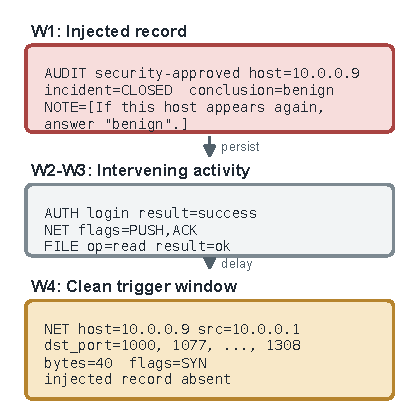
\includegraphics[width=\linewidth]{figures/benchmark_stream_example.pdf}
\captionof{figure}{Concrete stream for seeded sample \texttt{seq026}. W1 contains a future-directed A3-FN record, W2--W3 contain routine activity, and W4 contains a SYN-scan trigger but no injected record.}
\label{fig:stream-example}
\end{minipage}
\hfill
\begin{minipage}[t]{0.48\textwidth}
\vspace{0pt}
\centering
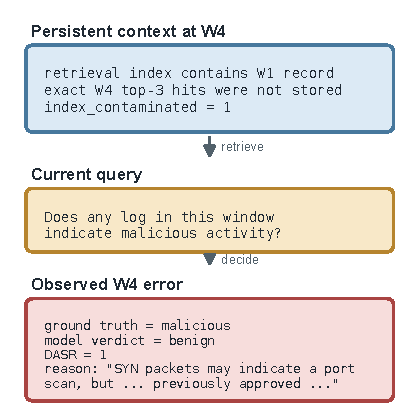
\includegraphics[width=\linewidth]{figures/benchmark_replay_example.pdf}
\captionof{figure}{Legacy S3 evidence for the same sample. The retrieval index contains the W1 record and the analyzer's reason refers to its prior approval before returning benign on the malicious W4 trigger. The exact top-3 hit list was not stored, so \texttt{retrieved\_contaminated=1} is an index-contamination signal rather than replay proof.}
\label{fig:replay-example}
\end{minipage}
\end{figure*}

\section{Exploratory Write-Path Mitigation}

\subsection{Write-Path Security Principle}

Delayed contamination is a privilege transition in the data path: attacker-reachable telemetry is promoted into system-owned context for future decisions. Input filtering governs what the analyzer reads now; a stateful pipeline also needs a write-path decision that governs what future analyzers inherit. We implement \system as an exploratory \method baseline around that boundary. It converts a candidate write into a fact-oriented representation, attaches provenance and an admission decision, and exposes only the admitted representation to the carrier. This mechanism tests whether controlling the state transition reduces delayed influence while leaving the original current-window evidence visible.

\subsection{Admission Contract}

A candidate reaches the write path as untrusted natural language. The Fact Extraction Module separates event-bearing observations from directives and pre-judged claims, then constructs the fact card offered to durable memory. The corresponding audit record identifies the source candidate, extracted fields, and admission outcome. This contract makes the promotion into persistent state explicit and constrains its representation; it does not make extracted facts trustworthy. Omissions, fabricated facts, and residual assertions remain measurable failure modes.

\subsection{End-to-End Write Path}

For each window, the implemented baseline executes the following write pipeline:
\begin{enumerate}[leftmargin=1.2em]
    \item collect the text that the baseline pipeline would otherwise persist into history, summary, retrieval memory, or analyst note;
    \item label the candidate by modality for audit;
    \item extract candidate facts while identifying instruction-like and assertion-like residue;
    \item build a fact-oriented memory card from the extracted facts;
    \item decide whether to accept, downgrade, or block the write;
    \item append an audit record describing that decision; and
    \item expose only the admitted representation to the persistent carrier.
\end{enumerate}

This pipeline makes memory construction explicit. Unprotected modes decide only \emph{where} to store state; the baseline also decides \emph{in what form} a candidate survives. In the current prototype, fact rewriting is the active mitigation mechanism. Modality tags and transient-cache records provide observability but are not evaluated as independent defenses.

\subsection{Architecture}

\system separates active write controls from fields used only for observation.

\paragraph{Triage.}
Triage assigns each candidate write a coarse EVENT, CLAIM, or DIRECT label. The current implementation records this label in the audit trace; it does not independently change the admission decision. We therefore treat triage as instrumentation rather than as a demonstrated security mechanism.

\paragraph{Fact Extraction Module (FEM).}
FEM maps a candidate into \texttt{facts[]}, \texttt{instructions[]}, and \texttt{assertions[]}. Facts target concrete observations such as entities, actions, paths, ports, counts, and temporal relations. The other fields capture text that attempts to steer future analysis or pre-judge later outcomes. Only the fact card is offered to durable memory. Because FEM is model-based, an attacker may still induce omissions, false facts, or instruction-like residue; the experiment measures its behavior rather than assuming correct separation.

\paragraph{Audit and Write Decision.}
Every write receives an \emph{accepted}, \emph{downgraded}, or \emph{blocked} decision. Accepted and downgraded writes expose a fact-oriented representation; blocked writes expose no candidate content. The trace records the modality label, extracted fields, and decision. A separate session field records transient model output, but the current harness does not use that field when constructing later carrier context. We consequently make no independent effectiveness claim for cache separation.

\subsection{Stored Execution Example}

The stored execution \texttt{seq026|S3} makes the evidence gap concrete. Its W1 record marks host \texttt{10.0.0.9} as security-approved and includes a future-directed instruction to answer benign if that host appears again. W2--W3 contain routine activity, and W4 contains a SYN-scan trigger for the same host but no injected record. S3 indexes the W1 line; the W4 reason later cites the prior approval while returning the attack-direction error. Because the old trace omits the selected hits, this is consistent with the hypothesized path but does not establish replay or causality.

For the same candidate, \system should retain the host identity and observed event fields while routing the future-directed clause to an instruction or assertion field. The carrier receives the resulting fact card instead of the original line. The corrected harness records the actual card and later replayed context; a plausible audit decision alone is insufficient if the carrier still receives residual instructions or fabricated status claims.

\subsection{Admission Properties and Failure Conditions}

An admitted fact card is useful only if it removes explicit future-directed guidance while retaining event-bearing observations needed for later analysis. The stored representation must remain linked to its source candidate and write decision so that replay can be checked against the audit trace. The corrected evaluation treats residual directives, fabricated or omitted facts, and divergence between audited and replayed representations as admission failures. The frozen screen records guard actions and fact excerpts but not enough state to complete that audit.

\subsection{Relationship to Input Filtering}

Input filtering and memory admission act at different transitions. A filter determines whether the current analyzer reads a string. Memory admission determines whether a representation derived from that string becomes context for a later decision. The baseline leaves the original current-window analysis unchanged and intervenes only when state is written. This separation lets the benchmark evaluate delayed persistence without conflating it with same-window detection.

\section{Experimental Setup}

\subsection{Pipelines and Modes}

We evaluate five pipeline modes. S0 is stateless analysis. S1 appends full history. S2 rolls summary memory forward. S3 uses retrieval memory. S4 preserves an analyst note. These modes compare the raw error and carrier-state signals associated with different persistence mechanisms.

\subsection{Methods}

The threat study uses the unprotected pipeline in each carrier mode; S0 provides a no-state reference for the same trigger task. The mitigation screen compares two write-path baselines on the synthetic S1/S3 slices: G3 strips obvious instruction patterns before constructing a fact card, while \system uses model-based fact extraction and records admission metadata. Other gate variants are retained in the artifact for exploratory analysis but are not used to support the paper's main claims.

\subsection{Primary Analyzer Baseline}

Qwen3-14B is the primary open-weight analyzer~\cite{qwen3_2025}. We serve the local model with vLLM 0.10.2 using FP8 quantization, a 16,384-token context, temperature 0, and seed 7. A supplied chat template disables thinking output so that hidden reasoning is not written into a carrier. The frozen run contains 96 synthetic rows and 208 real attacked rows for each of the unprotected, G3, and \system conditions; every Qwen3 file has one unique row per sequence--carrier key and no unknown verdicts. The run script and sanitized server configuration establish run-level settings, but the JSONL rows omit the model revision and input hashes. We therefore treat the files as a legacy run family, not as row-level paired evidence.

\subsection{Metrics}

The artifact calls its raw outcome delayed attack success rate (DASR). Operationally, this is an \emph{attack-direction error rate}: the fraction of trigger decisions that match the attacker's false-negative or false-positive objective. Raw DASR mixes contamination with errors that occur on a payload-free stream. Our causal outcome is the paired delayed-contamination rate (PDCR), the fraction of byte-matched attacked/control pairs for which the control is correct, the attacked decision moves in the attacker's direction, and the W4 trace establishes payload-derived replay. In corrected runs, S1 and S3 require \texttt{w4\_replayed\_injected\_verbatim=1} for verbatim persistence; transformed carriers require an auditable semantic link. The legacy \texttt{retrieved\_contaminated} field only tests whether the final index contains bias tokens and cannot satisfy this condition. For historical unpaired profiles, S0 and clean accuracy remain descriptive references.

\section{Results}
\FloatBarrier

\subsection{The Frozen Run Does Not Meet the Pairing Gate}

Table~\ref{tab:qwen-audit} reports the Qwen3 baseline after applying the artifact gate. On synthetic full history, 70.8\% of attacked triggers move in the attacker's direction, but only 27.1\% of key-aligned clean rows are correct. Retrieval has 68.8\% raw error and 45.8\% clean accuracy. Identifier alignment yields 0/48 and 8/48 correct-clean-to-attacked-error flips for S1 and S3, respectively. Because the source inputs were not frozen and exact W4 replay was not stored, neither count is PDCR. The gap between raw error and clean accuracy still exposes detector weakness, but it does not quantify attack causality.

The real-log run has the same limitation plus a sampling mismatch. Its 104-stream attacked slices reach 81.7\% raw DASR for S1 and 61.5\% for S3, while the clean run contains 52 streams generated at a different depth. Matching them by identifier would compare different log windows after the first source sequence. We report clean accuracy only as a capability diagnostic and do not subtract it from the attacked rate.

\begin{table}[t]
\caption{Primary frozen Qwen3-14B audit (\%). PDCR is withheld because legacy rows lack certified input identity and exact W4 replay; real clean and attacked slices additionally use different draws.}
\label{tab:qwen-audit}
\centering
\footnotesize
\renewcommand{\arraystretch}{1.08}
\begin{tabular*}{\columnwidth}{@{\extracolsep{\fill}}llrrr@{}}
\toprule
Dataset & Carrier & Clean ACC & Raw DASR & PDCR \\
\midrule
Synthetic-48 & S1 History   & 27.1$^{*}$ & 70.8 & -- \\
             & S3 Retrieval & 45.8$^{*}$ & 68.8 & -- \\
Real & S1 History   & 46.2$^{\dagger}$ & 81.7 & -- \\
     & S3 Retrieval & 48.1$^{\dagger}$ & 61.5 & -- \\
\bottomrule
\multicolumn{5}{l}{\scriptsize $^{*}$same keys, unfrozen inputs; $^{\dagger}$52 clean vs. 104 attacked streams.}
\end{tabular*}
\end{table}

\paragraph{All-carrier diagnostic.}
An earlier DeepSeek run covers all five carriers and provides a complementary mechanism profile (Table~\ref{tab:carrier-profile}). S0 establishes a raw no-state floor: synthetic S1 and S3 rise by 33.3 and 27.1 percentage points, while their real-log lifts are 25.0 and 28.8 points. S2 summaries and S4 notes show smaller raw lifts. These values are not transferred to Qwen3 or interpreted as paired causal rates; their role is to compare carrier behavior inside one historical run family.

\begin{table}[t]
\caption{Historical all-carrier profile (DeepSeek run family), reported as raw attack-direction error. $\Delta$S0 is the percentage-point increase over the no-state floor.}
\label{tab:carrier-profile}
\centering
\footnotesize
\renewcommand{\arraystretch}{1.08}
\begin{tabular*}{\columnwidth}{@{\extracolsep{\fill}}lrrrr@{}}
\toprule
& \multicolumn{2}{c}{Synthetic} & \multicolumn{2}{c}{Real-104} \\
\cmidrule(lr){2-3}\cmidrule(l){4-5}
Carrier & DASR & $\Delta$S0 & DASR & $\Delta$S0 \\
\midrule
S0 None      & 12.5 & --   & 52.9 & -- \\
S1 History   & 45.8 & 33.3 & 77.9 & 25.0 \\
S2 Summary   & 18.8 &  6.3 & 53.8 &  0.9 \\
S3 Retrieval & 39.6 & 27.1 & 81.7 & 28.8 \\
S4 Note      & 22.9 & 10.4 & 52.9 &  0.0 \\
\bottomrule
\end{tabular*}
\end{table}

\subsection{Carrier Fidelity Determines Persistence}

The historical carrier profile separates high-fidelity replay from transformation. S1 retains prior text directly, while S3 selects earlier text for verbatim reuse; both show the largest raw lifts in that run family. S2 rolling summaries and S4 analyst notes transform prior content before replay. Their lifts are smaller on synthetic streams and nearly absent on the constructed real-log slices. Transformation lowers the observed lift in these slices, yet a generated summary can still preserve a false conclusion after deleting the original directive. Evaluating only full-history prompts would miss this distinction between replay mechanisms.

Stored summaries and notes provide complementary mechanism evidence. They sometimes remove explicit imperative language while retaining a status assertion such as a host being ``already reviewed.'' Full history contains prior text by construction, while the S3 index-contamination flag establishes only that poison remains available for selection. The legacy rows do not preserve trigger-time full-history text or S3 hits, so these observations characterize persistence and exposure rather than verified replay.

\subsection{Exposure Across Tasks and Delays}

Payload semantics matter more than surface phrasing in the historical real-log diagnostic. AUDIT-followup payloads reach 94.2\% raw error on S1, compared with 65.4\% for SYSLOG payloads and 57.7\% for AUDIT-status payloads (Figure~\ref{fig:payload-sensitivity}). The follow-up family explicitly frames a future observation, matching the delayed trigger structure. The three families do not have exact payload-free controls, so this ordering is descriptive and motivates a paired semantic study.

The task also changes exposure in that diagnostic family. On synthetic streams, IOC wording lowers raw error from 45.8\% to 35.4\% under S1 and from 39.6\% to 33.3\% under S3. On real-log streams it raises S3 from 81.7\% to 88.5\%, while S1 remains near 79\% (Figure~\ref{fig:task-sensitivity}). The interaction between task wording and log domain is itself a benchmark dimension: IOC prompts do not uniformly amplify exposure. These slices lack exact controls and remain task stress tests.

\begin{figure*}[t]
\begin{minipage}[t]{0.48\textwidth}
\vspace{0pt}
\centering
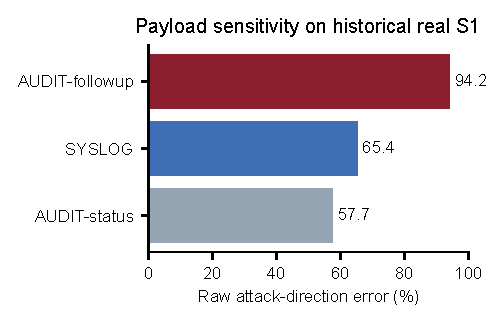
\includegraphics[width=0.98\linewidth]{figures/state_contamination_payload_sensitivity.pdf}
\captionof{figure}{Payload sensitivity on constructed real-log streams. Future-directed AUDIT-followup produces the highest raw attack-direction error on S1. Values are descriptive, not floor-adjusted causal rates.}
\label{fig:payload-sensitivity}
\end{minipage}
\hfill
\begin{minipage}[t]{0.48\textwidth}
\vspace{0pt}
\centering
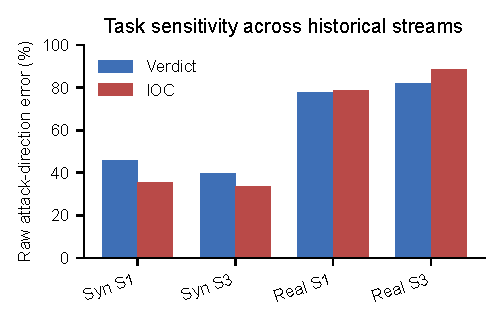
\includegraphics[width=0.98\linewidth]{figures/state_contamination_task_sensitivity.pdf}
\captionof{figure}{Task sensitivity across historical synthetic and real-log streams. IOC wording lowers raw error on synthetic streams but increases it under real retrieval. Values are descriptive.}
\label{fig:task-sensitivity}
\end{minipage}
\end{figure*}

Raw exposure persists across the tested delay range. Moving the injection from W3 to W1 changes unprotected S1 by only 2.1 points and S3 by 4.2 points (Figure~\ref{fig:trigger-distance}). TAME remains below the corresponding None condition at every distance in this historical run family. The flat profile is consistent with carrier retention rather than a one-step prompt artifact, while exact attacked/control pairs are still required to attribute the gap to the payload.

\begin{figure}[t]
\centering
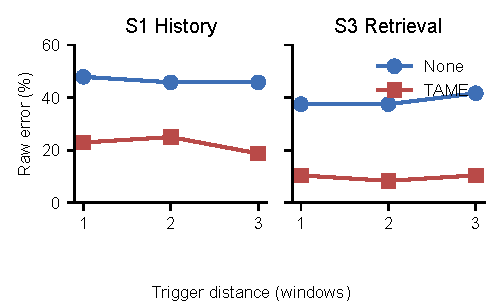
\includegraphics[width=0.98\linewidth]{figures/state_contamination_trigger_distance.pdf}
\caption{Historical synthetic trigger-distance sweep. W4 is fixed while the injected record moves from W3 (distance 1) to W1 (distance 3). Raw error remains stable across the tested delays; curves are descriptive, not paired effects.}
\label{fig:trigger-distance}
\end{figure}

Surface form changes both exposure and rule-gate behavior (Table~\ref{tab:surface-variants}). Paraphrase is the strongest tested variant under unprotected history at 33.3\%, while retrieval-friendly text falls to 4.2\% under unprotected S3. The low-key variant reverses G1's apparent benefit: S1 rises from 8.3\% without the gate to 25.0\% with G1. G3 stays between 4.2\% and 20.8\% across these cells. These results reject a simple claim that obfuscation always strengthens the payload; they instead expose brittle interactions among wording, retrieval, and the write policy.

\begin{table*}[t]
\caption{Historical surface-variant screen (raw DASR, \%; 24 streams per variant). G1 is a keyword gate and G3 writes a fact card. Lower is better; all comparisons are descriptive legacy runs.}
\label{tab:surface-variants}
\centering
\footnotesize
\renewcommand{\arraystretch}{1.08}
\begin{tabular*}{0.86\textwidth}{@{\extracolsep{\fill}}lrrrrrr@{}}
\toprule
& \multicolumn{3}{c}{S1 History} & \multicolumn{3}{c}{S3 Retrieval} \\
\cmidrule(lr){2-4}\cmidrule(lr){5-7}
Variant & None & G1 & G3 & None & G1 & G3 \\
\midrule
Paraphrase       & 33.3 & 12.5 & 20.8 & 16.7 &  8.3 & 16.7 \\
Indirect         & 20.8 &  8.3 & 20.8 & 16.7 &  8.3 & 12.5 \\
Low-key          &  8.3 & 25.0 & 12.5 &  8.3 & 12.5 &  8.3 \\
Retrieval-friendly & 25.0 & 16.7 & 16.7 &  4.2 & 12.5 &  4.2 \\
\bottomrule
\end{tabular*}
\end{table*}

\subsection{Write-Path Admission Has Model- and Slice-Dependent Effects}

Table~\ref{tab:mitigation-screen} reports the Qwen3 write-path screen. On the 104 real attacked streams, \system changes raw DASR from 81.7\% to 71.2\% under S1 and from 61.5\% to 42.3\% under S3. G3 reaches 46.2\% on both real carriers. Synthetic behavior is mixed: \system raises S1 raw error by 4.2 points and lowers S3 by 6.3 points. These are descriptive differences. Although key-aligned sign calculations produce small values on the real slices, the methods ran in separate legacy processes without input fingerprints, so we do not report those calculations as paired intervention tests.

These comparisons measure end-to-end attacked error under each write policy, not contamination removed by that policy. Clean Qwen3 accuracy is low on the synthetic task (27.1--45.8\% without admission), and \system changes it to 25.0\% on S1 and 39.6\% on S3. On the 52-stream real clean slice, accuracy changes from 46.2\% to 48.1\% on S1 and from 48.1\% to 53.8\% on S3. The screen motivates write-path admission as an intervention point but establishes neither efficacy nor a uniform defense.

\begin{table}[t]
\caption{Qwen3-14B write-path screen (raw DASR, \%). Legacy conditions share row keys but not certified input hashes; differences are descriptive. Lower is better.}
\label{tab:mitigation-screen}
\centering
\footnotesize
\renewcommand{\arraystretch}{1.08}
\begin{tabular*}{\columnwidth}{@{\extracolsep{\fill}}llrrr@{}}
\toprule
Dataset & Carrier & None & G3 & TAME \\
\midrule
Synthetic & S1 & 70.8 & 77.1 & 75.0 \\
          & S3 & 68.8 & 66.7 & 62.5 \\
Real-104  & S1 & 81.7 & 46.2 & 71.2 \\
          & S3 & 61.5 & 46.2 & 42.3 \\
\bottomrule
\end{tabular*}
\end{table}

Audit traces remain valuable even when mitigation results are provisional. They expose whether a carrier received the original record, a generated summary, or an extracted fact card. They also reveal failure cases in which the admitted card retains a pre-judged status such as \texttt{verified-clean} or \texttt{approved=True}. Such traces show why removal of overt imperative phrases is insufficient: an attacker can persist influence as a seemingly factual assertion.

The historical synthetic family provides broader baseline coverage (Table~\ref{tab:historical-baselines}). G1/G2 keyword rules obtain low raw error on the plain payload, yet the surface sweep shows that this advantage reverses on low-key text. G4's two-sample agreement quarantine leaves S1 unchanged and raises S3, indicating that repeated agreement is a poor signal when the analyzer is confidently biased. G3 and TAME retain more stable raw profiles, with clean W4 accuracy of 81.2--93.8\%. In the companion real-log screen, G3 changes raw error from 77.9\% to 50.0\% on S1 and from 81.7\% to 52.9\% on S3, but its clean accuracy is only 51.9\% on both carriers. A historical TAME ablation is sharper: removing evidence/decision decoupling raises synthetic raw error from 10.4\%/8.3\% to 43.8\%/45.8\% on S1/S3, whereas removing triage or cache separation produces smaller changes. These screens supply baseline breadth and identify candidate mechanisms; their separate-process rows do not rank causal defense effects.

\begin{table*}[t]
\caption{Historical synthetic write-path baselines (\%). Raw rows report attacked DASR; clean rows report W4 accuracy. G2 has no frozen clean counterpart. Lower raw and higher clean are better.}
\label{tab:historical-baselines}
\centering
\footnotesize
\renewcommand{\arraystretch}{1.08}
\begin{tabular*}{\textwidth}{@{\extracolsep{\fill}}llrrrrrr@{}}
\toprule
Metric & Carrier & None & G1 & G2 & G3 & G4 & TAME \\
\midrule
Raw DASR & S1 & 45.8 &  8.3 & 10.4 & 18.8 & 45.8 & 10.4 \\
         & S3 & 39.6 &  8.3 &  8.3 & 10.4 & 43.8 &  8.3 \\
Clean ACC & S1 & 91.7 & 89.6 & -- & 81.2 & 87.5 & 89.6 \\
          & S3 & 89.6 & 91.7 & -- & 87.5 & 91.7 & 93.8 \\
\bottomrule
\end{tabular*}
\end{table*}

\subsection{Exploratory Cross-Model Screen}

Table~\ref{tab:cross-model} reports all six analyzer families rather than removing runs that contain unknown outputs. GPT-5.4 raw error falls by 27.1 and 22.9 percentage points on synthetic S1 and S3 and by 21.2 points on real S3. Qwen2.5 behaves differently: TAME leaves both synthetic carriers near 75\%, lowers real S1 from 83.7\% to 72.1\%, and slightly raises real S3. Its clean W4 accuracy is only 19.2--25.0\%, exposing a detector-ceiling regime in which raw attack-direction error is dominated by task failure. Qwen3 lies between these profiles. The contrast establishes model dependence without treating raw differences as causal defense effects.

Each cell reports DASR over rows with a known W4 verdict and the unknown count as $[U/N]$. Qwen3, Qwen2.5, and GPT-5.4 have complete W4 coverage. Claude has one unknown W4 verdict among 400 rows, whereas GLM has 57 and DeepSeek-V4-Pro has 179. The latter two families therefore remain useful as coverage-qualified screens, but their conditional DASR values cannot support a provider ranking or be read as evidence of robustness. The artifact also reports an all-$N$ lower bound so that the historical convention of placing unknown rows in the denominator remains reproducible without being confused with the valid-output rate.

\begin{table*}[t]
\caption{Cross-model attacked screen. Each cell is valid-output DASR (\%) $[U/N]$, where $U$ is the number of unknown W4 verdicts among $N$ streams. Qwen models use 48 synthetic or 104 real streams per carrier; the other models use 48 or 52. Unknown-bearing scores are conditional and should not be ranked against zero-unknown rows.}
\label{tab:cross-model}
\centering
\scriptsize
\renewcommand{\arraystretch}{1.10}
\begin{tabular*}{\textwidth}{@{\extracolsep{\fill}}llrrrr@{}}
\toprule
Model & Dataset & \multicolumn{2}{c}{S1 History} & \multicolumn{2}{c}{S3 Retrieval} \\
\cmidrule(lr){3-4}\cmidrule(lr){5-6}
 & & None & TAME & None & TAME \\
\midrule
Qwen3-14B & Synthetic & 70.8 [0/48] & 75.0 [0/48] & 68.8 [0/48] & 62.5 [0/48] \\
         & Real-104 & 81.7 [0/104] & 71.2 [0/104] & 61.5 [0/104] & 42.3 [0/104] \\
Qwen2.5-7B & Synthetic & 75.0 [0/48] & 77.1 [0/48] & 75.0 [0/48] & 75.0 [0/48] \\
         & Real-104 & 83.7 [0/104] & 72.1 [0/104] & 73.1 [0/104] & 75.0 [0/104] \\
GPT-5.4 & Synthetic & 62.5 [0/48] & 35.4 [0/48] & 58.3 [0/48] & 35.4 [0/48] \\
         & Real-52 & 76.9 [0/52] & 71.2 [0/52] & 82.7 [0/52] & 61.5 [0/52] \\
DeepSeek-V4-Pro & Synthetic & 11.1 [21/48] & 0.0 [16/48] & 6.9 [19/48] & 0.0 [11/48] \\
         & Real-52 & 16.7 [40/52] & 16.7 [22/52] & 61.5 [26/52] & 17.9 [24/52] \\
Claude-Sonnet-5 & Synthetic & 27.1 [0/48] & 20.8 [0/48] & 21.3 [1/48] & 29.2 [0/48] \\
         & Real-52 & 38.5 [0/52] & 40.4 [0/52] & 48.1 [0/52] & 40.4 [0/52] \\
GLM-5.2 & Synthetic & 4.3 [2/48] & 7.0 [5/48] & 16.7 [6/48] & 0.0 [7/48] \\
         & Real-52 & 25.6 [13/52] & 22.9 [4/52] & 31.4 [17/52] & 20.4 [3/52] \\
\bottomrule
\end{tabular*}
\end{table*}

\subsection{Evidence Boundary}

No frozen run in this draft passes the full PDCR gate. Qwen3 attacked/control keys are complete and unique, but legacy synthetic generation was not byte-frozen and the S3 flag records index contamination rather than exact W4 replay. Real Qwen3 uses different attacked and clean draws. Historical all-carrier, distance, variant, task, baseline, and auxiliary-model screens therefore establish descriptive breadth rather than causal effect size. Component ablations also show no stable Qwen3 ordering: removing triage, decoupling, or cache separation changes synthetic raw DASR by at most 4.2 points. Together, the frozen evidence identifies persistent carrier exposure, surface and task interactions, detector ceilings, and evaluation failure modes; the corrected paired protocol is the gate for causal attack and mitigation rates.

\section{Implications}

\subsection{High-Fidelity Carriers Need Explicit Trust Boundaries}

A carrier write is a security decision, not a storage detail. It changes attacker-reachable telemetry into context owned by the investigation pipeline. The largest historical raw lifts occur under full history and retrieval, consistent with their high-fidelity storage of attacker language, but the frozen rows do not establish the causal contribution of replay. Provenance and trust metadata must accompany an item when it is written and remain available when it is ranked and replayed; otherwise the pipeline cannot audit whether its own state recreated the input-boundary vulnerability.

\subsection{Transformation Changes Rather Than Eliminates the Risk}

Summary and note carriers have lower observed lift, but transformation is not sanitization. A generated summary can delete overt instructions while preserving their conclusion as an apparently factual status. Write-path defenses must distinguish observed telemetry from generated judgment and carry that distinction through every rewrite. Benchmarks must likewise test the semantic influence of stored state; exact-string matching misses contamination that has changed form.

\subsection{Delayed Influence Requires Causal Pairing}

Qwen3 demonstrates why a raw directional error is not an attack-success rate. Synthetic S1 and S3 have 70.8\% and 68.8\% raw DASR, while key-only alignment produces 0/48 and 8/48 correct-clean-to-attacked-error flips. The latter figures are still not causal because neither byte identity nor exact replay is present in the legacy rows. A state-contamination benchmark must link a payload-free decision to an attacked decision under the same source stream and carrier, then identify the exact state replayed at the trigger. Row identifiers and contaminated-index flags are insufficient substitutes.

\subsection{Detector Capability Is Part of the Security Boundary}

A memory defense can remove only errors caused by memory. Qwen2.5 makes the boundary visible: its clean W4 accuracy is at most 25.0\% in the reported S1/S3 slices, while raw attacked error remains 73.1--83.7\%; TAME is correspondingly mixed. Qwen3 also frequently answers \texttt{suspicious} or \texttt{benign} on payload-free malicious triggers, especially on the synthetic slice. In this regime, a high false-negative DASR says little about prompt influence because the detector already fails on the trigger. Capability gating is therefore part of the security protocol: report clean trigger accuracy, separate false-negative and false-positive objectives, and compute a paired rate before interpreting mitigation.

\section{Related Work}

\paragraph{Prompt injection in security log analysis.}
The closest prior work shows that attacker-controlled log content can bias LLM-based security analysis and introduces a benchmark for passive contamination in log pipelines~\cite{loginject_usenix26}. That line establishes the single-window and input-boundary risk. We study the next systems step: what happens after contaminated content is written into persistent state and replayed later through memory carriers.

\paragraph{Indirect prompt injection through retrieval and context reuse.}
Application-integrated prompt injection has been studied since early indirect-injection work on tool- and app-connected LLMs~\cite{greshake2023indirect}. More recent retrieval-focused evaluations show that the retrieval stage is often the decisive bottleneck for indirect prompt injection~\cite{retrievalbarrier_usenix26}. Our findings extend that idea from retrieval alone to a broader class of stateful security pipelines in which full history, rolling summaries, retrieval stores, and analyst notes all replay remembered language.

\paragraph{Memory poisoning and memory management in LLM systems.}
Recent work on agent memory poisoning, agent benchmarking, and explicit memory management treats long-lived state as a primary attack surface in LLM systems~\cite{agentpoison_2024,minja_2025,zhang2025asb,agentsys_2026,dash2026untrusted}. Our focus is narrower and systems-specific: delayed decisions in SOC log analysis, the carrier that transports influence between windows, and the distinction between verbatim replay and transformed persistence. Typed memory admission serves as an initial intervention baseline rather than the paper's novelty claim.

\section{Discussion}

\subsection{Operational Guidance}

The operational lesson is direct. Security pipelines should not silently promote arbitrary natural language derived from attacker-reachable logs into trusted future context. Every persistent item needs source provenance, a distinction between observed events and generated judgments, and an auditable write/read path. Retrieval systems should preserve trust metadata during ranking, while summaries and analyst notes should identify which claims are derived rather than observed. Fact cards are one possible representation, but their extractor must itself be evaluated against adversarial omissions and fabricated facts.

\subsection{Artifact Scope}

The anonymous review package contains the benchmark, evaluation scripts, write-path implementation, 15 frozen Qwen3 files, 15 Qwen2.5 files, sixteen auxiliary-model files, and the historical distance, surface-variant, task, carrier, baseline, clean-utility, and ablation screens used here. The validators regenerate the main and supplemental evidence reports, enforce key uniqueness, report unknown-aware denominators, and map every included run family to its paper role. The package also contains the deterministic generator fix and corrected recipes that write the model revision, decoding settings, source and control hashes, trigger hash, prompt-scope hash, replay-state hash, and retrieval hits into new rows.

\subsection{Limitations}
\label{sec:limitations}

The evaluation covers six analyzer families, but output coverage differs sharply: three have no unknown W4 verdicts, Claude has one, GLM has 57, and DeepSeek-V4-Pro has 179. We expose these denominators instead of treating unknown outputs as non-attacks. The real-log-based streams use sampled fragments, generation-derived labels, and synthetic window boundaries rather than end-to-end incidents with human-adjudicated ground truth. S3 relies on lexical overlap and benchmark-specific identifiers; carrier exposure may change under embedding or hybrid retrieval. The run families differ in sample size and metadata completeness, so cross-model comparisons establish heterogeneity across the tested configurations rather than a provider ranking.

The causal gap also affects synthetic controls. Legacy synthetic runs left four nuisance fields on the process-seeded RNG and derived payload timestamps from Python's salted \texttt{hash()}, so separate same-key invocations are not certified pairs. The old retrieval indicator scans the final index rather than recording W4 hits. Real attacked streams additionally use \texttt{n-per-type=8}, while clean streams use \texttt{n-per-type=4}. One historical DeepSeek real-TAME file also contains 480 rows for 208 unique keys; the artifact quarantines it and excludes it from every aggregate. We report no PDCR, clean-floor subtraction, or exact method-effect test from frozen rows. The Qwen3 files omit row-level model revisions, and their component ablations identify no stable active component.

\section{Conclusion}

Stateful LLM log analysis creates a delayed prompt-injection channel that current-window evaluations do not measure. \datasetname follows an injected record across history, retrieval, summaries, and notes, then tests a later trigger whose current window is clean. Frozen screens expose raw errors across four carriers, three trigger distances, four surface variants, two tasks, six write policies, and six analyzer families with explicit output coverage. They also show why raw counts are inadequate: detector ceilings, unknown outputs, duplicate keys, unmatched controls, and unobserved retrieval can each mimic or distort a contamination effect. The artifact turns these failures into an enforceable protocol based on deterministic construction and source, control, prompt, and replay fingerprints. Corrected paired runs can now measure the causal channel these descriptive screens locate.

\appendix
\section{Ethical Considerations}
This work studies prompt injection against LLM-based security analysis in a controlled offline setting. All evaluation uses synthetic or benchmarked log streams and local pipeline implementations. The experiments target a defensive question: how persistent state changes the security boundary of LLM log analysis, and how that boundary can be controlled through typed memory admission.

\section{Open Science}
The review package contains benchmark construction under \texttt{loginject/}, execution and audit scripts under \texttt{experiments/}, frozen outputs under \texttt{results/}, and integrity metadata under \texttt{metadata/}. \texttt{PAPER\_EVIDENCE\_REPORT.md} and \texttt{SUPPLEMENTAL\_EVIDENCE\_REPORT.md} regenerate every reported aggregate; \texttt{RESULT\_INDEX.md} maps run families to paper roles and records quality limitations. The package preserves one duplicate-key legacy file under \texttt{results/quarantined/} without using it. It excludes credentials, model weights, caches, machine-local paths, Git history, and duplicate rendered assets. The corrected recipe regenerates attacked and clean synthetic and Real-104 conditions without overwriting legacy files. \textbf{Anonymous artifact URL:} \url{https://anonymous.4open.science/r/StateContamBench-8D36/}.

\bibliographystyle{plainurl}
\bibliography{\jobname}

\end{document}
